\subsection{Теорема Лиувилля}
\begin{flalign*}
	\dv x = \v f(\v x) \quad (1)
\end{flalign*}
\begin{df}
	\[
		V = \int \ldots \int dx_1 \ldots dx_n 
	\]
	--- фазовый объем.
\end{df}
\begin{df}
	$\v x_0 \rightarrow \v x = \v x(t, \v x_0)$ --- фазовый поток системы $(1)$.
\end{df}
\begin{teo}
	Если $\Div f = 0$, то $V = const$.
\end{teo}
\begin{proof}
	\begin{flalign*}
		& \v x = \v x_0 + t\v f(\v x_0) + O_2(t) &\\
		& V = \int \ldots \int dx_1 \ldots d x_n = \int \ldots \int \abs{\det \pd{\v x}{\v x_0}} dx_{10}\ldots dx_{n0} &\\
		& \det \pd{\v x}{\v x_0} = \det\left( E + t\pd{\v f(\v x_0)}{\v x_0} + O_2 \right) = 1 + t \tr\left( \pd{\v f(\v x_0)}{\v x_0} \right) + O_2 &\\
		& \dot V \vert_{t = 0} = \int \ldots \int \left(0 + \tr \left(\pd{\v f(\v x_0)}{\v x_0}\right) + O_2\right) dx_{10}\ldots dx_{n0} \qquad\qquad \begin{vmatrix}
			1 + t\pd{f_1}{x_{10}} & \overbrace{t\cdot(*)}^{O_2} \\
			t \cdot (-*) & 1 + t\pd{f_2}{x_{20}} \\
		\end{vmatrix} &\\
		& \tr \pd{\v f(\v x_0)}{\v x_0} = 0 \Rightarrow \dot V \vert_{t = 0} = 0 &\\
		& \Div \v f = \sum\pd{f_i}{x_i} = 0 \Rightarrow \dot V \vert_{t = t_*}, \; \forall t_* \Rightarrow V = const &\\
	\end{flalign*}
\end{proof}
\begin{flalign*}
	& \begin{cases}
		\dot q = \pd{H}{p} \\
		\dot p = -\pd{H}{q} \\	
	\end{cases}
	\begin{array}{l}
		\v x = (q_1,\ldots, q_n, p_1,\ldots, p_n)^T \\
		\v f_H = \left( \pd{H}{p_1},\ldots,\pd{H}{p_n}, -\pd{H}{q_1},\ldots,-\pd{H}{q_n} \right) \\
	\end{array}
	&\\
	& \Div \v f_H = \sum_{i = 1}^n \frac{\partial^2H}{\partial q_i \partial p_i} - \sum\limits_{i = 1}^n\frac{\partial^2 H}{\partial p_i\partial q_i} = 0 \Rightarrow V_h = const 
\end{flalign*}
\begin{ntc}
	Такие преобразования фазов. пот. сохраняют $V$.
\end{ntc}

\subsection{Обратные теоремы теории интегральных инвариантов}
\begin{teo}
	Если на любой трубке траектории системы дифференциальных уравнений вида
	\[
		\begin{cases}
			\dot q = Q(q,\; p,\; t) \\
			\dot p = P(q,\; p,\; t)	\\
		\end{cases}
		\quad (*)
	\]
	$I_\text{п} = \oint\limits_{C:t = const} (p, \delta q)$ сохраняется, то данная система гамильтонова.
\end{teo}
\begin{proof}
	\begin{flalign*}
		& \frac{d}{dt}I_\text{п} = \oint\limits_{C: t = const}(\dot p, \delta q) + (p, \delta \dot q) = \oint\limits_{C: t =const} \delta(p, \dot q) - (\delta p, \dot q) + (\dot p, \delta q) \overset{(*)}{=} &\\
		& = \oint\limits_C(P, \delta q) - (Q, \delta p) = 0 \quad \forall C \Leftrightarrow \exists H: (P, \delta q) - (Q, \delta p) = -\delta H = -\left( \pd{H}{p}, \delta p \right) - \left( \pd{H}{q}, \delta q \right) &\\
		& Q = \pd{H}{p},\; P = -\pd{H}{q} &\\
	\end{flalign*}
\end{proof}
\begin{teo}
	Если на любой трубке прямых путей системы $(*)$ $I_\text{пк} = \oint\limits_C (p, dq) - Hdt$, то система гамильтонова с гамильтонианом $H$.
\end{teo}
\begin{proof}
	Возьмем $C_1$, на котором $dt = 0$(изохроны).
	\begin{flalign*}
		& \oint\limits_C(p, dq) - Hdt = \oint\limits_{C_1}(p, dt) \text{ --- инвариант} \Rightarrow \text{ по предыдущей теореме } \exists H(q,\; p,\; t): \begin{cases}
			\dot q = \pd{H^*}{p} \\
			\dot p = -\pd{H^*}{q} \\
		\end{cases}
		\Rightarrow &\\
		& \Rightarrow I_\text{пк}^* = \oint\limits_C(p, dq) - H^*dt = \oint\limits_{C_1}(p, dq) &\\
		& I_\text{пк} - I_\text{пк}^* = \oint\limits_C (H^* - H)dt = 0 \quad \forall C \Leftrightarrow (H^* - H)dt = dF = \left( \pd{F}{q}, dq \right) + \left( \pd{F}{p}, dp \right) + \pd{F}{t}dt &\\
		& \pd{F}{q} = \pd{F}{p} = 0,\; \pd{F}{t} = H^* - H &\\
		& \begin{cases}
			\pd{H}{p} = \pd{H^*}{p} \\
			\pd{H}{q} = \pd{H^*}{q} \\
		\end{cases}
		\Rightarrow
		\text{ система $(*)$ гамильтонова с гамильтонианом $H$.} &\\
	\end{flalign*}
\end{proof}

\subsection{Канонические преобразования}
\begin{flalign*}
	& (1)\begin{cases}
		\dot q = \pd{H}{p} \\
		\dot p = -\pd{H}{q} \\
	\end{cases} \quad
	(2)\begin{cases}
		\tilde q = \tilde q(q,\; p,\; t) \\
		\tilde p = \tilde p(q,\; p,\; t) \\
	\end{cases}
	\Leftrightarrow
	\begin{cases}
		q = q(\tilde q, \tilde p, t) \\
		p = p(\tilde q, \tilde p, t) \\
	\end{cases} &\\
	& H = H(q, p, t) \qquad \det \pd{(\tilde q, \tilde p)}{(q, p)} \neq 0 &\\
	& \dot{\tilde q}\vert_{(1)} = \left.\left( \pd{\tilde q}{q}\dot q + \pd{\tilde q}{p}\dot p + \pd{\tilde q}{t} \right)\right|_{(1)} = Q(\tilde q,\; \tilde p,\; t) \overset{?}{=} \pd{\tilde H}{\tilde p} &\\
	& \dot{\tilde p}\vert_{(1)} = \left.\left( \pd{\tilde p}{p}\dot p + \pd{\tilde p}{p}\dot p + \pd{\tilde p}{t} \right)\right|_{(1)} = P(\tilde q,\; \tilde p,\; t) \overset{?}{=} -\pd{\tilde H}{\tilde q} &\\
\end{flalign*}
\begin{xmp}
\begin{flalign*}
	& H = \frac{p^2 + q^2}{2},\; \begin{cases}
		\tilde q = p^2 \\
		\tilde p = q \\
	\end{cases}
	\quad
	\begin{cases}
		q = \tilde p \\
		p = \pm \sqrt{\tilde q} \\
	\end{cases} &\\
	& \begin{cases}
		\dot q = \pd{H}{p} = p \\
		\dot p = -\pd{H}{q} = -q \\
	\end{cases} \qquad
	\begin{array}{ll}
		\dot{\tilde q} = 2p\dot p = -2pq = \mp2\tilde p \sqrt{\tilde q} & \overset{?}{=} Q = \pd{\tilde H}{\tilde p} \\
		\dot{\tilde p} = p = \pm\sqrt{\tilde q} & \overset{?}{=} P = -\pd{\tilde H}{\tilde q} \\
	\end{array} &\\
	& \pd{Q}{\tilde q} = \pd{P}{\tilde p} \qquad \mp \tilde p \cdot \frac{1}{\sqrt{\tilde q}} \neq 0 \Rightarrow \text{ система не гамильтонова.}
\end{flalign*}
\end{xmp}
\begin{df}
	Неособенное (т.е. обр.) преобразование вида $(2)$ называется каноничным, если оно \emph{любую} гамильтонову систему превращает в гамильтонову систему.
\end{df}
\begin{teo}[Критерий канонического преобразования] 
	Преобразование $(2)$ каноническое $\Leftrightarrow \exists c \neq 0,\; F(q, p, t)$:
	\[
		(\tilde p, d\tilde q) - \tilde Hdt = c((p, dq) - Hdt) - dF
	\]
\end{teo}
\begin{proof}
	\ovalbox{$\Rightarrow$}
	\begin{figure}[H]
		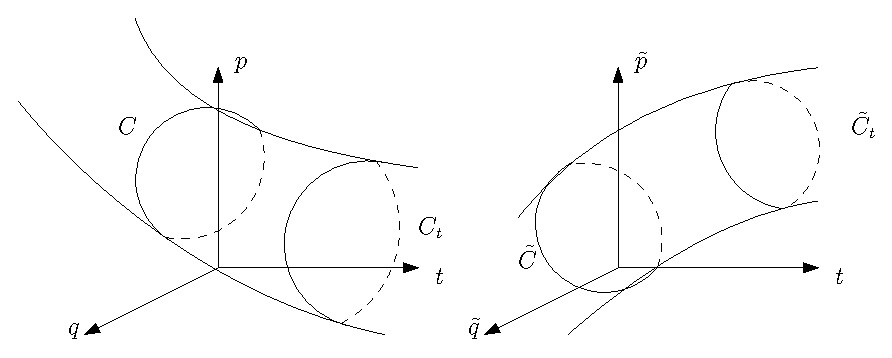
\includegraphics{10_1.eps}
	\end{figure}
	\begin{flalign*}
		& C \xrightarrow{(2)} \tilde C &\\
		& \oint\limits_{\tilde C}(\tilde p, d \tilde q) - \tilde Hdt = \oint\limits_{\tilde C: t = const} (\tilde p, \delta \tilde q), \qquad\begin{array}{l}
			\tilde p = \tilde p(q,\; p,\; t) \\
			\tilde q = \tilde q(q,\; p,\; t) \\
		\end{array} &\\
		& \oint\limits_C(\tilde p, d\tilde q) - \tilde Hdt = \oint\limits_{C_t} \left( \tilde p, \pd{\tilde q}{q}\delta q + \pd{\tilde q}{p} \delta p \right) = \oint\limits_{C_t}(A, \delta q) - (B, \delta p) \overset{\text{т. Ли-Хуанчжуна}}{=} &\\
		& = c\oint\limits_{C_t}(p, \delta q) = \left( \oint\limits_C(p, dq) - Hdt \right)c &\\
		& \oint\limits_C\left( (\tilde p, d\tilde q) - \tilde Hdt - c[(p, dq) - Hdt]\right) = 0 \quad \forall C \Leftrightarrow (\tilde p, d\tilde q) - \tilde Hdt = c((p, dq) - Hdt) - dF &\\
	\end{flalign*}
	\ovalbox{$\Leftarrow$} Проинтегрируем равенство
	\begin{flalign*}
		& \oint\limits_C (\tilde p, d\tilde q) - \tilde Hdt = c\oint\limits_C(p, dq) - Hdt - \underbrace{\oint df}_{0} = I &\\
		& \oint\limits_{C} (\tilde p, d\tilde q) - \tilde Hdt = \oint\limits_{\tilde C} (\tilde p, d\tilde q) - \tilde Hdt \text{ --- инвариант, т.к. $I$ --- инвариант.} &\\
		& \text{По второй обратной теореме система гамильтонова с гамильтонианом $\tilde H$.} &\\
	\end{flalign*}
\end{proof}
\begin{df}
	$c = const \neq 0$ --- валентность преобразования, $F(q,\; p,\; t)$ --- производящая функция.
\end{df}
